\documentclass[border=5pt]{standalone}
\usepackage{tikz}
\usepackage{amsmath}

\begin{document}
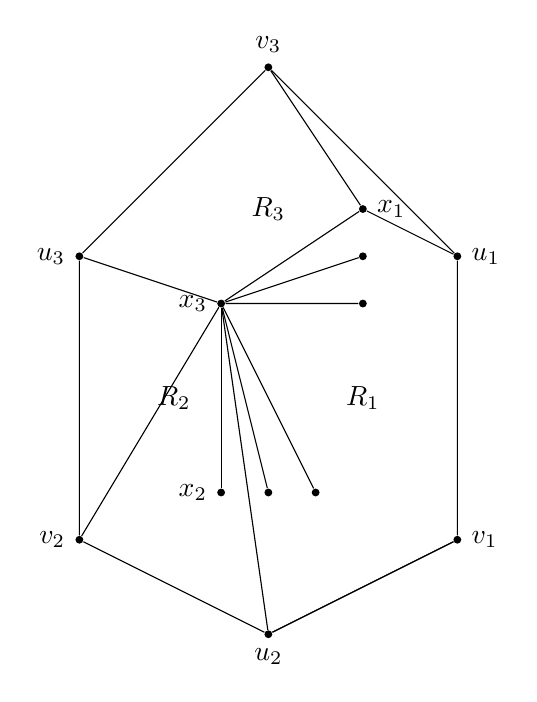
\begin{tikzpicture}[scale=1.2]

% 定义顶点样式
\tikzset{vertex/.style={circle, fill, inner sep=1pt}}

% 绘制外部框架顶点
\node[vertex, label={left:$u_3$}] (u3) at (0,3) {};
\node[vertex, label={left:$v_2$}] (v2) at (0,0) {};
\node[vertex, label={below:$u_2$}] (u2) at (2,-1) {};
\node[vertex, label={right:$v_1$}] (v1) at (4,0) {};
\node[vertex, label={right:$u_1$}] (u1) at (4,3) {};
\node[vertex, label={above:$v_3$}] (v3) at (2,5) {};

% 绘制内部顶点
\node[vertex, label={right:$x_1$}] (x1) at (3,3.5) {};
\node[vertex, label={left:$x_3$}] (x3) at (1.5,2.5) {};
\node[vertex, label={left:$x_2$}] (x2) at (1.5,0.5) {};

% 未标记的内部顶点
\node[vertex] (i1) at (3,3) {};
\node[vertex] (i2) at (3,2.5) {};
\node[vertex] (i3) at (2,0.5) {};
\node[vertex] (i4) at (2.5,0.5) {};

% 区域标记
\node at (3,1.5) {$R_1$};
\node at (1,1.5) {$R_2$};
\node at (2,3.5) {$R_3$};

% 绘制外部框架线条
\draw (u3) -- (v3) -- (u1) -- (v1) -- (u2) -- (v2) -- (u3);
\draw (u3) -- (x3) -- (v2);
\draw (u1) -- (x1) -- (v3);
\draw (v1) -- (u2);

% 绘制内部连接
\draw (x3) -- (x1);
\draw (x3) -- (i1);
\draw (x3) -- (i2);
\draw (x3) -- (x2);
\draw (x3) -- (i3);
\draw (x3) -- (i4);
\draw (x3) -- (u2);

\end{tikzpicture}
\end{document}